%!TEX root = /Users/louis/Documents/PhD/Deliverables/ProgressReport/pr.tex
\section{Progress}
\label{sec:progress}
I have made progress in four areas. Firstly, I have conducted a thorough review of literature in the areas of co-evolution and synchronisation, elaborating the aims of my research. Secondly, I have located examples of evolutionary changes in MDE projects. Thirdly, I have used the examples to evaluate existing techniques for managing evolutionary change in MDE. Fourthly, I have begun to develop a language for specifying evolution. In this section, the progress made in each of these areas is discussed in turn.

In my qualifying dissertation, the term \emph{case study} was used to describe an existing MDE project containing examples of evolution. In this report, the term \emph{example} is preferred.

%!TEX root = /Users/louis/Documents/PhD/Deliverables/ProgressReport/pr.tex
\subsection{Elaboration of Research Aims}
\label{sub:elaboration}
The aim of my research is to develop structures and processes for evolutionary changes in the context of Model-Driven Engineering. Since submitting my qualifying dissertation, I have identified two categories of evolutionary change (for which structures and processes can be developed) by reviewing literature relating to evolution in MDE. Both are discussed below.

\subsubsection{Model and Metamodel Co-Evolution} % (fold)
\label{ssub:model_and_metamodel_co_evolution}
A metamodel is a collection of concepts that are used for specifying models in a particular domain. A model and metamodel are \emph{consistent} when the metamodel specifies every concept used in the model definition. Consistency can be described by a set of constraints between models and metamodels \cite{paige07metamodel}. When all constraints are satisfied, a model and a metamodel are consistent. For example, the Eclipse Modelling Framework\footnote{The Eclipse Modelling Framework (EMF) \cite{steinberg09emf} provides tools for developing, managing and instantiating metamodels.} specifies many constraints for checking model and metamodel consistency: one such constraint is that every object in the model has a corresponding non-abstract class in the metamodel.

A metamodel can evolve (be adapted by a developer), which can cause inconsistency. For example, suppose a concept is removed from a metamodel. Any models that use the removed concept are now inconsistent with the metamodel. \emph{Co-evolution} is the process of evolving both metamodel and model such that they remain consistent. In existing approaches for managing co-evolution (such as \cite{herrmannsdoerfer08cope,cicchetti08automating}), metamodel evolution occurs first, possibly causing models to become inconsistent. Any inconsistent models are then evolved to re-establish consistency.


\subsubsection{Model Synchronisation} % (fold)
\label{ssub:model_synchronisation}
Often, MDE is used to generate code from a model. The MDA guidelines suggest beginning by defining a platform-independent model, and using at least one transformation to produce platform-specific model(s). Code is then generated from the final platform-specific model. When one model evolves, the changes need to be propagated to other models. This activity is termed \textit{model synchronisation}.

Existing model synchronisation literature focuses mostly on enabling \textit{incremental transformation}, a style of model transformation that incrementally updates the target model. For large models, transformation execution time has been shown to be significantly reduced by using incremental transformation \cite{hearnden06incremental}. However, \cite{kolovos08scalability} suggests that building models that are less monolithic (using modularisation) is likely to yield better results than attempting to develop techniques for scaling up model management tasks (such as model transformation). Consequently, I argue that the focus of existing model synchronisation literature is misplaced; model synchronisation research should seek to improve maintainability rather than just simply scalability.  %TODO : read Dimitrios's paper and make this argument strong; "likely to yield better results" is inspecific and weak

Although much of the model synchronisation literature concentrates on incremental transformation, there are other closely-related areas of research, which are more relevant to my work. For instance, \cite{jouault05loosely,drivalos08loosely} describe models of traceability, which could be used to perform \textit{impact analysis} (highlighting the consequences of performing an evolutionary change). Eclipse's Java Development Tools project successfully employs impact analysis for illustrating the effects of Java refactorings \cite{fuhrer07refactoring}. I am unaware of any existing work that explores implementing impact analysis for MDE tools.
%!TEX root = /Users/louis/Documents/PhD/ProgressReport/pr.tex
\subsection{Locating Examples of Evolution}
In my qualifying dissertation, I identified the need for categorising the ways in which MDE development artefacts evolve over time. The categorisation will be used to provide requirements for developing structures and processes for evolutionary changes in the context of model-driven engineering.

A study of example data (existing MDE projects containing evolution) was proposed to produce this categorisation. Work has progressed by defining requirements for candidates for the study. Existing MDE projects were located and analysed against the requirements. Finally, the most suitable candidate projects were selected. As will be discussed in Section \ref{sub:analysis_of_existing_techniques}, the selected projects have been used to analyse existing techniques for managing evolution in MDE.

\subsubsection{Requirements} % (fold)
\label{ssub:requirements}
The requirements defined for candidates for the study of evolution are presented below. In Section \ref{sub:elaboration}, two categories of evolutionary change were identified: model and metamodel co-evolution; and model synchronisation. I wanted to study both. Consequently, requirements were partitioned into three types: those necessary for studying each of the two categories of evolutionary change, and common requirements (applicable to both categories of evolutionary change).

\paragraph{Common requirements}
Every candidate project had to use some aspect of MDE, such as metamodelling or model transformation (requirement R1). In addition, each candidate project had to provide historical information, which elucidated the evolution of development artefacts (R2). For example, several versions of the project from the source code management system. Finally, a candidate project had to contain a sizeable number of significant changes\footnote{`Sizeable' and `significant' are deliberately vague. Further details are given in Section \ref{ssub:project_selection}.} (R3).

\paragraph{Model and metamodel co-evolution}
A candidate project for the study of model and metamodel co-evolution had to define a metamodel and some changes to that metamodel (R4). In the projects considered, the metamodel changes took the form of either (1) another version of the metamodel, or (2) a history (which recorded each of the steps used to produce the adapted metamodel).

A candidate project also had to provide example instances of models before and after each migration activity (R5).

Ideally, a candidate project included more than one consecutive metamodel adaptation, so as to represent the way in which the same development artefacts can continue to evolve over time (optional requirement O1).

\paragraph{Model synchronisation}
A candidate project for the study of model synchronisation had to define a model-to-model transformation (R6).

Furthermore, a candidate project had to include many examples of source and target model for that transformation (R7).

Crucially, a candidate project had to provide many examples of the kinds of change (to either source or target model) that cause inconsistency between the models (R8). 

Ideally, a candidate project also included transformation chains (more than one model-to-model transformation, executed sequentially) (O2). Chains of transformations are prescribed by the MDA guidelines \cite{kleppe03mda}.

% subsubsection requirements (end)

\subsubsection{Project Selection} % (fold)
\label{ssub:project_selection}
Eight candidates were considered for the study. Table \ref{tab:candidates} shows which of the requirements (defined above) are fulfilled by each of the candidates. Each candidate is now discussed in turn.

\begin{table}
	\caption{Candidates for study of evolution in existing MDE projects}
	\centering
	\begin{tabular}{|c||c|c|c||c|c|c||c|c|c|c|}
		\hline
		\multirow{3}{*}{Name} & \multicolumn{10}{|c|}{Requirements} \\
		\cline{2-11}
		          & \multicolumn{3}{|c||}{Common} & \multicolumn{3}{|c||}{Co-evolution} & \multicolumn{4}{|c|}{Synchronisation} \\
		\cline{2-11}
		          & R1 & R2 & R3 & R4 & R5 & O1 & R6 & R7 & R8 & O2 \\
		\hline
		GSN       & x  &    &    & x  &    &    &    &    &    &    \\
		\hline
		Watson    & x  &    &    & x  &    &    & x  &    &    &    \\
		\hline
		Zoos      & x  & x  &    & x  &    &    &    &    &    &    \\
		\hline
		MDT       & x  & x  &    & x  &    & x  &    &    &    &    \\
		\hline
		ModelPlex & x  & x  & x  & x  &    & x  & x  & x  &    &    \\
		\hline
		FPTC      & x  & x  & x  & x  & x  &    &    &    &    &    \\
		\hline
		xText     & x  & x  & x  & x  & x  & x  & x  & x  &    & x  \\
		\hline
		GMF       & x  & x  & x  & x  & x  & x  & x  & x  &    & x  \\
		\hline
	\end{tabular}
	\label{tab:candidates}
\end{table}

\paragraph{GSN} % (fold)
\label{par:gsn}
Georgios Despotou and Tim Kelly are constructing a metamodel for Goal Structuring Notation (GSN). The metamodel has been developed incrementally. There is no accurate and detailed version history for the GSN metamodel (requirement R2). \textbf{Suitability for study:} Unsuitable.
% paragraph gsn (end)

\paragraph{OMG} % (fold)
\label{par:omg}
Andrew Watson references the development of two MDE projects in \cite{watson08mdahistory}. I emailed Watson to ascertain whether the source code for the studies was available. Source code was available for one of the projects, but there is no version history. \textbf{Suitability for study:} Unsuitable.
% paragraph omg (end)

\paragraph{Zoos} % (fold)
\label{par:zoos}
There are several collections of popular metamodels available in \emph{zoos}. Each zoo contains metamodels authored in one metamodelling language (e.g. EMF's Ecore). I considered two zoos for this study, but neither contained any significant metamodel changes. Those changes that were made involved only renaming of meta-classes (trivial to migrate) or additive changes (which do not affect consistency, and therefore require no migration). \textbf{Suitability for study:} Unsuitable.
% paragraph zoos (end)

\paragraph{MDT} % (fold)
\label{par:mdt}
The Eclipse Model Development Tools (MDT) \cite{mdt} provides implementations of industry-standard metamodels, such as UML2 \cite{uml212} and OCL \cite{ocl2}. Like the metamodel zoos, the version history for the MDT metamodels contained no significant changes. \textbf{Suitability for study:} Unsuitable.
% paragraph mdt (end)

\paragraph{ModelPlex} % (fold)
\label{par:modelplex}
Jendrik Johannes has made available to me work from the European project, ModelPlex. Johannes's work involves transforming UML models to Tool Independent Performance Models (TIPM) for simulation. Although the TIPM metamodel and the UML-to-TIPM transformation have been changed significantly, no significant changes have been made to the models. \textbf{Suitability for study:} Unsuitable.
% paragraph modelplex (end)

\paragraph{FPTC} % (fold)
\label{par:fptc}
Failure Propagation and Transformation Calculus (FPTC) provides a means for reasoning about the failure behaviour of complex systems. Before starting my doctorate, I worked with Richard Paige to develop an implementation of FPTC in Eclipse. The implementation includes an FPTC metamodel. Recent work with Philippa Conmy identified a significant flaw in the implementation, leading to changes to the metamodel. These changes caused existing FPTC models to become inconsistent with the metamodel. Conmy has made available to me copies of FPTC models from before and after the changes. \textbf{Suitability for study:} Suitable for model and metamodel co-evolution. Unsuitable for studying model synchronisation.
% paragraph fptc (end)

\paragraph{xText} % (fold)
\label{par:xtext}
xText is an openArchitectureWare (oAW) \cite{oaw} tool for generating parsers, metamodels and editors for performing text-to-model transformation. Internally, xText defines a metamodel, which has been changed significantly over the last year. In several cases, changes have caused inconsistency with existing models (such as the ones used in the FPTC project). xText provides examples of use, which have been updated alongside the metamodel. \textbf{Suitability for study:} Suitable for studying model and metamodel co-evolution. Unsuitable for studying model synchronisation.
% paragraph xtext (end)

\paragraph{GMF} % (fold)
\label{par:gmf}
The Graphical Modelling Framework (GMF) \cite{gronback06gmf} allows the definition of graphical concrete syntax for metamodels that have been defined in EMF. GMF prescribes a model-driven approach: Users of GMF define concrete syntax as a model, which is used to generate a graphical editor. In fact, five models are used together to define a single editor using GMF.

GMF defines the metamodels for graphical, tooling and mapping definition models; and for generator models. The metamodels have changed considerably during the development of GMF. Some changes have caused inconsistency with GMF models. Presently, migration is encoded in Java. Gronback\footnote{Private communication, 2008.} has stated that the migration code is being ported to QVT (a model-to-model transformation language) as the Java code is difficult to maintain.

GMF fulfils almost all of the requirements for the study. A large amount of data for the co-evolution of metamodels and models is available, including migration strategies. The GMF source code repository does not contain examples of the kinds of change that cause inconsistency between the models. However, GMF has a large number of users, and it may be possible to gather this information elsewhere. \textbf{Suitability for study:} Suitable for studying both categories of evolutionary change.
% paragraph gmf (end)

\paragraph{Summary of selection}
The FPTC and xText projects were selected for a study of model and metamodel co-evolution. No appropriate projects were located for a study of model synchronisation. The GMF project will not be studied now, but reserved as a case study for evaluating my research.

\subsubsection{Other data} % (fold)
\label{ssub:other_data}
As only a small number of candidate projects fulfilled all of the requirements, I decided to collect additional data from alternative sources. Firstly, I sought examples from related domains (e.g. object-oriented systems) for suitable data. Secondly, I am collaborating with colleagues from two projects, both of which are using iterative and incremental model-driven development. Example data for both categories of evolutionary change will be available from these two projects.

\paragraph{Examples of evolution from object-oriented systems} % (fold)
\label{par:examples_of_evolution_from_object_oriented_systems}
In object-oriented programming, software is constructed by developing groups of related objects. Every object is an instance of (at least) one class. A class is a description of characteristics, which are shared by each of the class's instances (objects).

A similar relationship exists between models and metamodels: metamodels comprises meta-classes, which describe the characteristics shared by each of the meta-class's instances (elements of a model). Together, model elements are used to describe one perspective (model) of a system

Consequently, I believe that studying the evolution of object-oriented systems will yield results that are relevant to the model and metamodel co-evolution occurring in MDE. To support this argument, I have performed a preliminary study of frequently observed changes made to object-oriented systems.

\subparagraph{Preliminary study of object-oriented refactorings} % (fold)
\label{subp:preliminary_study_of_object_oriented_refactorings}
\emph{Refactoring} is the process of improving the structure of existing code while maintaining its external behaviour. When used as a noun, a refactoring is one such improvement. \cite{fowler99refactoring} provides a catalogue of refactorings for object-oriented systems. For each refactoring, Fowler gives advice and instructions for its application.

Fowler's refactorings provide examples of evolutionary changes to object-oriented systems. I attempted to apply each of Fowler's refactorings to EMF metamodels and discovered that some are irrelevant to metamodelling. Those refactorings that do not apply to EMF metamodels belong to one of three categories:

\begin{enumerate}
	\item \textbf{Operational refactorings} focus on restructuring behaviour (method bodies). EMF does not support the specification of behaviour in models.
	\item \textbf{Navigational refactorings} convert, for example, between bi-directional and uni-directional associations. These changes are non-breaking in EMF, which automatically provides values for the inverse of a reference when required.
	\item \textbf{Domain-specific refactorings} manage issues specific to object-oriented programming, such as casting, defensive return values, and assertions. These issues are not relevant to metamodelling.
\end{enumerate}

The object-oriented refactorings that can be applied to metamodels provide examples of metamodel evolution. When applied, some of these refactorings potentially cause inconsistency between a metamodel and its models. I used Fowler's description of each refactoring to deduce a migration strategy for updating (co-evolving) inconsistent models. An example of deducing a migration strategy is now presented.

Figure \ref{fig:refactoring} illustrates a refactoring that changes a reference object to a value object. Value objects are immutable, and cannot be shared (i.e. any two objects cannot refer to the same value object). Reference objects are mutable, and can be shared. Figure \ref{fig:refactoring} indicates that applying the refactoring restricts the multiplicity of the association (on the Order end) to 1 (implied by the composition); prior to the refactoring the multiplicity is many.

\begin{figure}[htbp]
  \begin{center}
    \leavevmode
    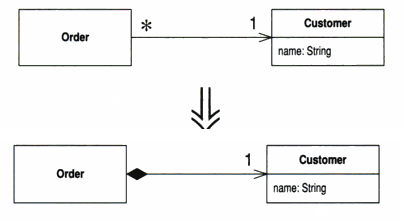
\includegraphics[scale=0.5]{refactoring.png}
  \end{center}
  \caption{Refactoring a reference to a value. Taken from \cite{fowler99refactoring}[pg183]}
  \label{fig:refactoring}
\end{figure}

Before applying the refactoring, each customer may be associated with more than one order. After the refactoring, each customer should be associated with only one order. Fowler indicates that every customer associated with more than one order should be duplicated, such that one customer object exists for each order. Therefore, the migration strategy in Listing \ref{lst:refactoring} is deduced.

\begin{lstlisting}[caption=Migration strategy for the refactoring in pseudo code., label=lst:refactoring]
for every customer, c
	for every order, o, associated with c
		create a new customer, d
		copy the values of c's attributes into d
	next o
	
	delete c
next c
\end{lstlisting}

Using this process, I deduced migration strategies for each of the refactorings that were (1) applicable to EMF metamodels, and (2) caused inconsistencies between a metamodel and its models. Since, I have recognised some of the metamodel changes in the FPTC project (one of the projects chosen for the model and metamodel co-evolution study) as object-oriented refactorings.

Object-oriented refactorings are used to improve the maintainability of existing systems. In other words, they represent only one of the three reasons for evolutionary change defined by \cite{sjoberg93quantifying}. The two other types of changes to object-oriented systems are equally relevant to my research. Consequently, I have obtained further examples of changes made to object-oriented systems from Tim Hoverd, an experienced object-oriented developer. Hoverd's examples include changes made that represent at least one of the other reasons for evolutionary change defined by \cite{sjoberg93quantifying}.

% subparagraph preliminary_study_of_object_oriented_refactorings (end)
% paragraph examples_of_evolution_from_object_oriented_systems (end)


\paragraph{Collaborations} % (fold)
\label{par:collaborations}
As well as locating example data from object-oriented programs, I am currently collaborating with two colleagues who are using MDE. Adam Sampson and I are constructing a metamodel to standardise the way in which his team model process-oriented programs. Heather Barber and I are investigating the feasibility of implementing a tool for generating story-worlds for interactive narratives.

In both cases, the work will involve constructing a metamodel for describing concepts in the domain. The metamodels will be developed incrementally, and consequently will change over time. In both cases, the domain is large, so I am hopeful that evolution will involve more than just additive changes. If so, the data will be used for studying model and metamodel co-evolution.

Both parties have expressed an interest in transforming their models to generate code (possibly via an intermediate model). If realised, the data will be used for studying model synchronisation.

% paragraph collaborations (end)
% subsubsection other_data (end)

\subsubsection{Summary}
To summarise, I have located eight existing MDE projects, three of which contain data that can be analysed to obtain requirements for the development of structures and process for evolutionary changes in the context of model and metamodel co-evolution occurring during model-driven engineering. One of the three projects, GMF, will be reserved as a case study for my thesis. Refactorings and other examples from object-oriented programming will supplement the data available from the existing MDE projects. Collaboration with Sampson and Barber will yield further data.

As I have been able to locate more examples of model and metamodel co-evolution than model synchronisation, I have decided to proceed by focusing on developing structures and processes for model and metamodel co-evolution. Should I discover further sources of model synchronisation, I will expand my research accordingly.





%!TEX root = /Users/louis/Documents/PhD/Deliverables/ProgressReport/pr.tex
\subsection{Analysis of Existing Techniques}
\label{sub:analysis_of_existing_techniques}


\subsubsection{Model and Metamodel Co-Evolution}
\begin{itemize}
	\item Introduce COPE and Cicchetti's work. I found them in the lit review discussed in Section \ref{sub:elaboration}. Mention that the literature did not demonstrate the use of the tools on real-world examples. 
	\item Explain my process for analysing these tools.
	\item Discuss the current status of my analysis.
\end{itemize}

    Analysed the most promising tools using data from a real-world system.

    Presented HUTN at MoDELs. At the same conference, a tool (called COPE) for managing model and metamodel co-evolution was presented. COPE makes use of a generic syntax for performing model migration and metamodel evolution.

%!TEX root = /Users/louis/Documents/PhD/Deliverables/ProgressReport/pr.tex
\subsection{Towards a Language for Automating Co-Evolution}
\label{sub:development}
Begun cataloguing types of model evolution. Started with Fowler's refactorings, and now expanding to incorporate evolutions seen in real-world systems.

